\section{Results}
\label{sec:Results}
The whole simulation setup and the methodology described in the last sections 
can be used to draw limits on the contribution of GRBs and other short 
transients to the detected diffuse high energy neutrino flux (HESE flux). The 
results and the impacts of different models is described in this section.

\subsection{Limits on Contribution to the HESE Flux by Transient Neutrino 
Sources}
In chapter \ref{sec:limits}, the methodology to calculate limits on the 
contribution of a transient population to the HESE flux was described. The 
pseudo experiments need to be repeated for each different signal model. The 
result for a spectrum with $\gamma=2.3$, 3000 GRBs per year and a fraction of 
5.95\% of the HESE flux to be produced by these GRBs are shown in Figures 
\ref{fig:test_statistic} and \ref{fig:test_statistic_cumulative}. The GRB rate 
density is not a known value but a parameter. To calculate the p-value for 
different rate densities and fraction of contribution to the HESE flux, the 
signal expectation $\mu_s$ can be scaled by 
\begin{equation}
 \hat{\mu_s} = \mu_s \cdot \zeta \frac{3000\mathrm{ 
GRBs/yr}}{N_\mathrm{GRBs/yr}}
\end{equation}
with $\zeta$ being the contribution to the total HESE flux. By doubling the 
number of GRBs, the neutrino flux per GRB gets reduced by half, leading to 
softer limits.

\begin{figure}[h]
 \centering
 \captionsetup{width=.9\textwidth}
%  \captionsetup{margin=0pt}
 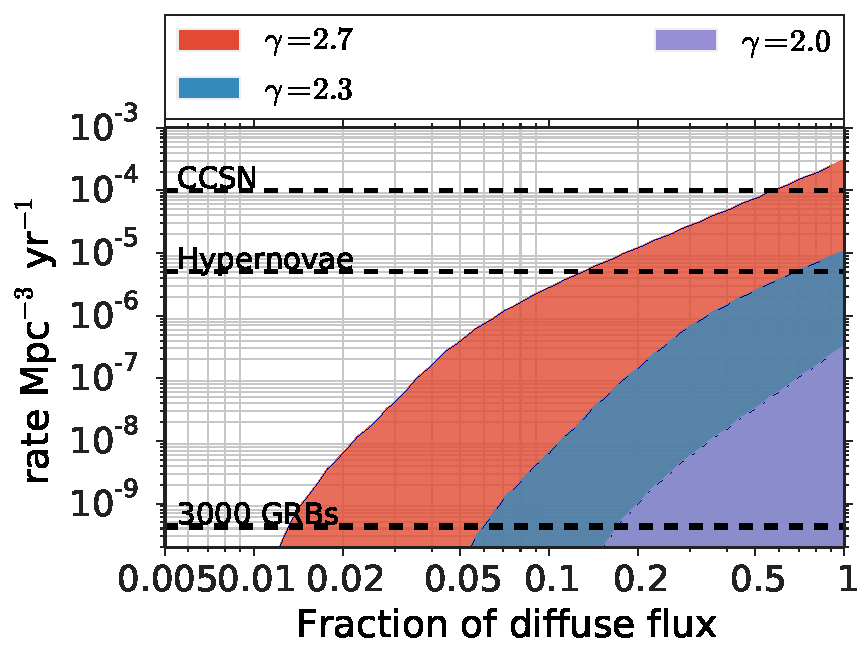
\includegraphics[width=0.75\textwidth]{fig/limits_wp_allgammas.pdf}
\caption{Limits on the contribution of short transient sources to the HESE 
flux depending on their rate density. The 90\% confidence regions are shown for 
three different spectra using the WP model.}
\label{fig:WP_2d_limit}
\end{figure}

Figure \ref{fig:WP_2d_limit} showcases the limits for the three different 
spectra using the WP model. The softer the spectrum the more singlets are 
expected especially at lower energies (Fig. \ref{fig:Espectra}) increase the 
multiplet expectation as well. Therefore, the hardest limits can be 
drawn using a spectrum with $\gamma=2.7$ decreasing in power the harder the 
spectrum gets. The results for a flux to be ruled out at a 90\% confidence 
level are listed in Table \ref{tab:WP_2d_limit_3000}.


\begin{table}[h]
  \centering
  \begin{tabular}{c|c|c}
$\gamma$  &  $N_\mathrm{GRB/yr}$ & $\zeta$ \\
\hline
2.7 & 3000 & 0.013 \\
2.3 & 3000 & 0.0595 \\
2.0 & 3000 & 0.18 \\
  \end{tabular}
  \caption{The values of the fraction to the HESE flux and the number of GRBs 
per year that are ruled out at a 90\% confidence level.}
  \label{tab:WP_2d_limit_3000}
\end{table}


\subsubsection{Signal origin}
% As part of the analysis, the question which simulated GRBs contribute most to 
% the limits, shall be answered in this section.
To answer the question on which GRBs the limits are most reliant on, the 
dependence on the luminosity and the redshift is examined at the 90\% 
confidence limit point for 3000 GRBs per year. Representing the different 
season and spectra, the BDT season and the intermediate spectrum with 
$\gamma=2.3$ were selected.

\begin{figure}[h!]
\centering
 \captionsetup{width=.9\textwidth}
%  \captionsetup{margin=0pt}
\subfloat[WP model\label{fig:ngrb_redshift_dependence_swiftdoublet_ndetF}]{%
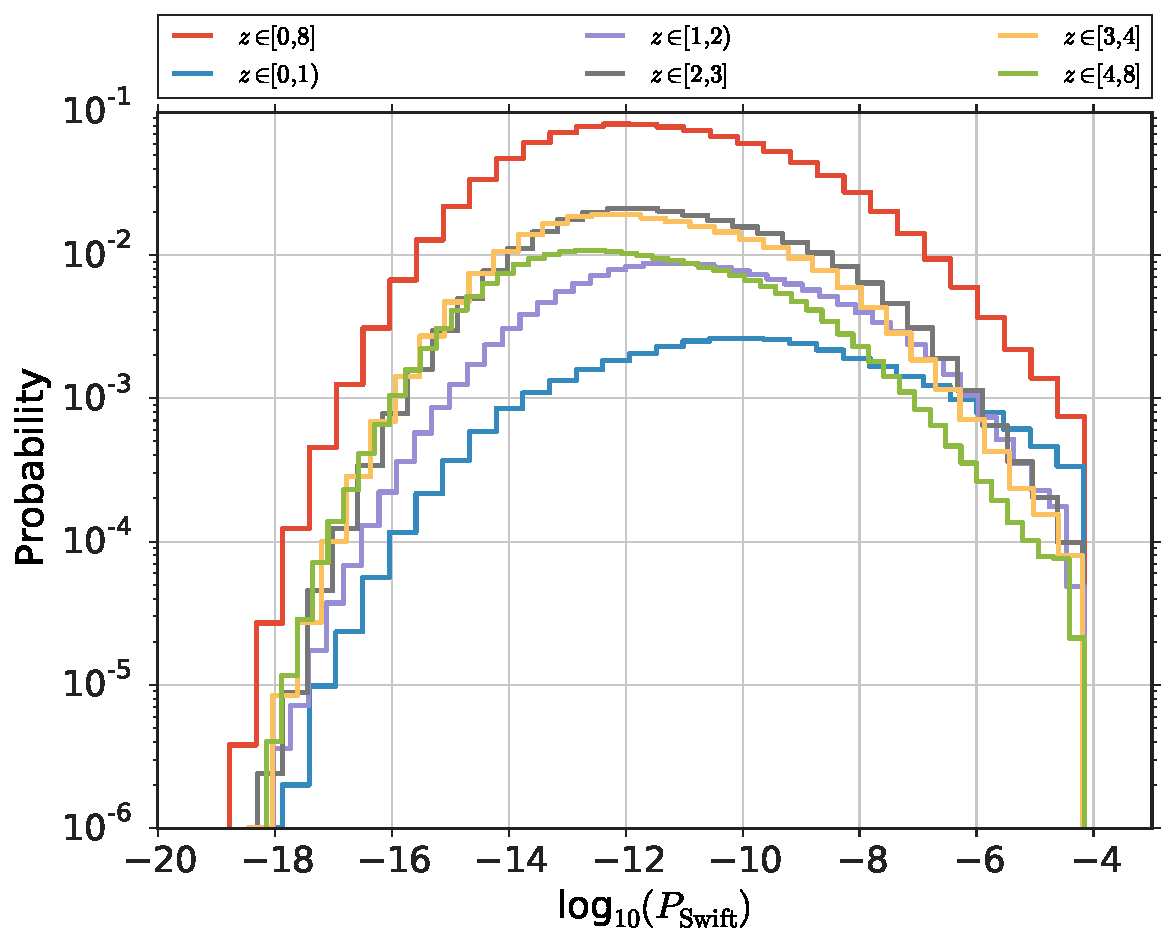
\includegraphics[width=0.45\textwidth]{%
fig/ngrb_redshift_dependence_swiftdoublet_ndetF.pdf}}
\subfloat[HC model\label{
fig:ngrb_hc_redshift_dependence_swiftdoublet_ndetF}]{%
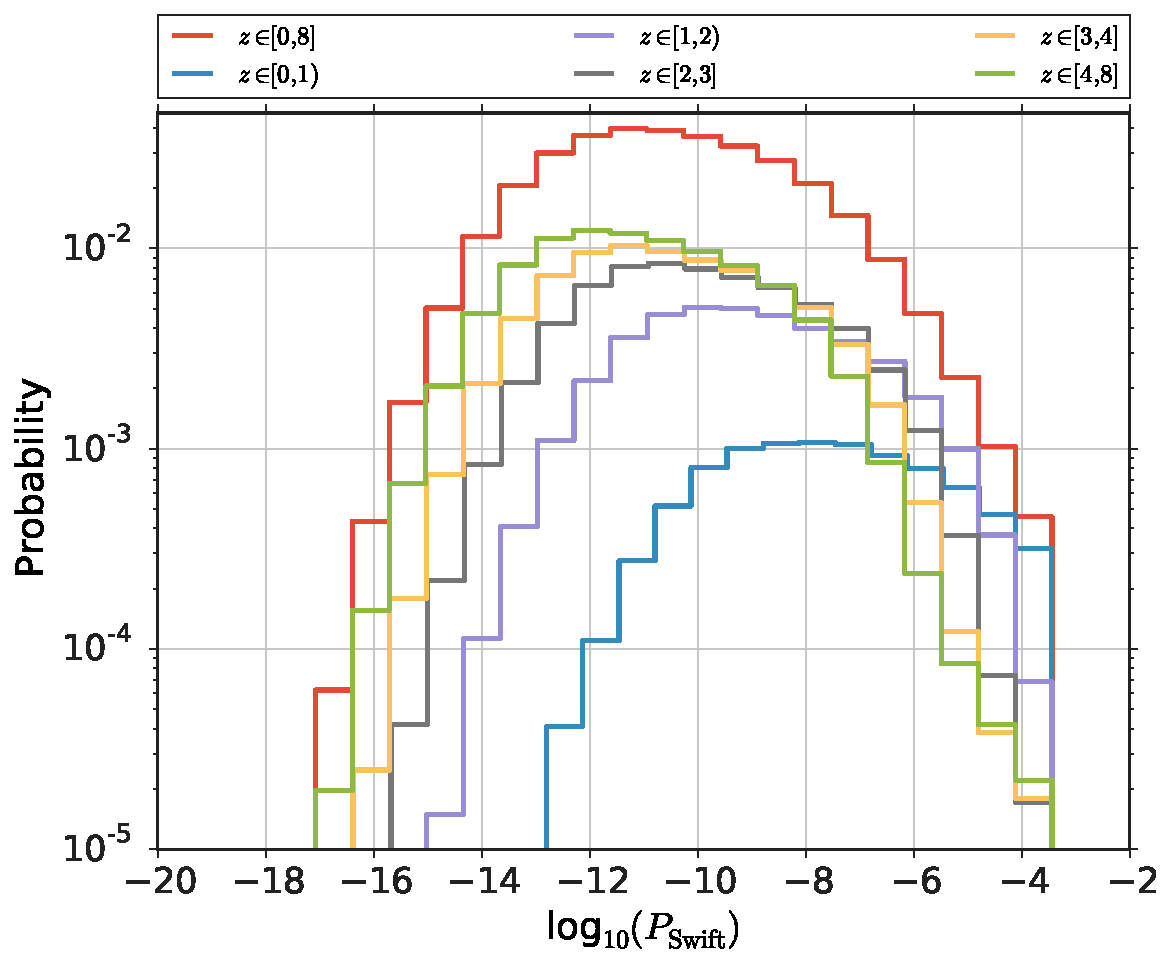
\includegraphics[width=0.45\textwidth]{%
fig/ngrb_hc_redshift_dependence_swiftdoublet_ndetF.pdf}}\\
\subfloat[WP model\label{fig:ngrb_lum_dependence_swiftdoublet_ndetF}]{%
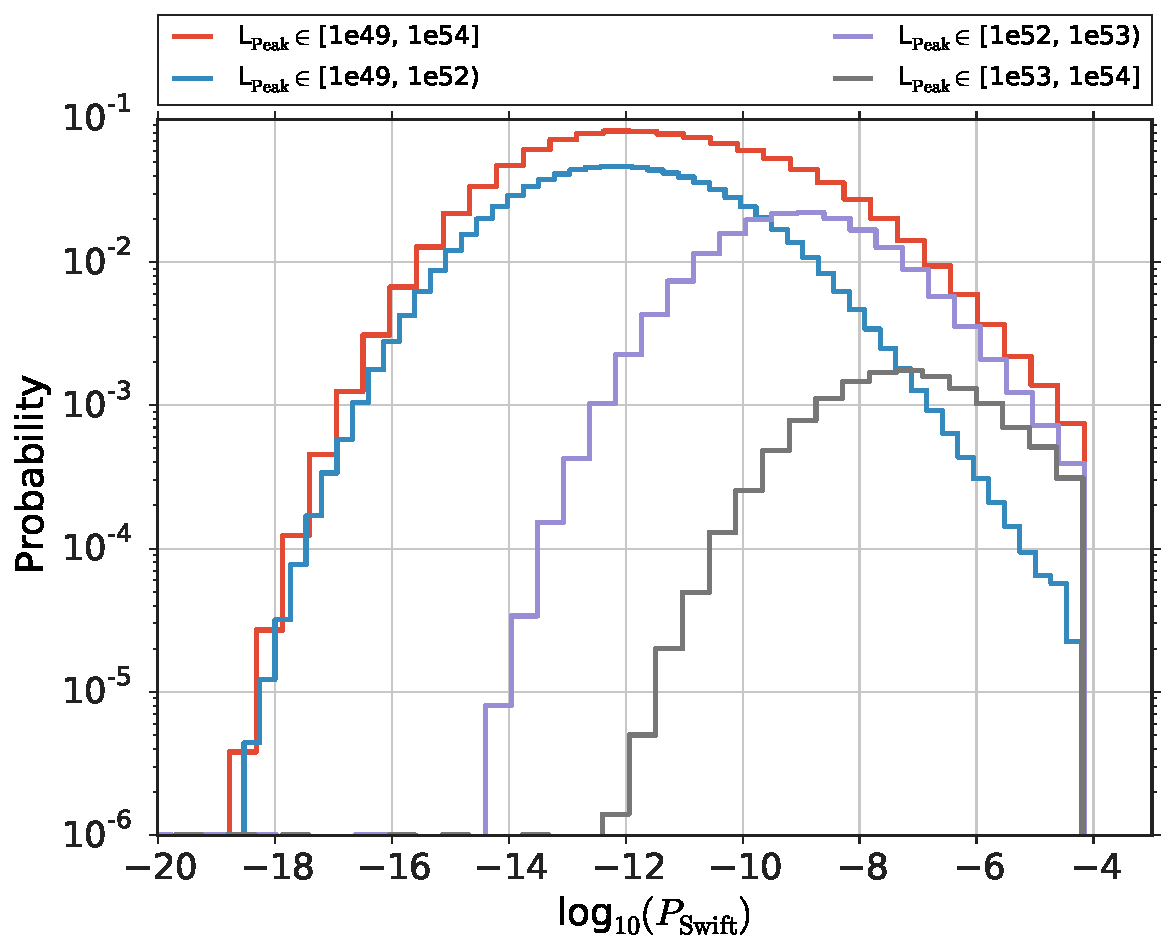
\includegraphics[width=0.45\textwidth]{%
fig/ngrb_lum_dependence_swiftdoublet_ndetF.pdf}}
\subfloat[HC model\label{fig:ngrb_hc_lum_dependence_swiftdoublet_ndetF}]{%
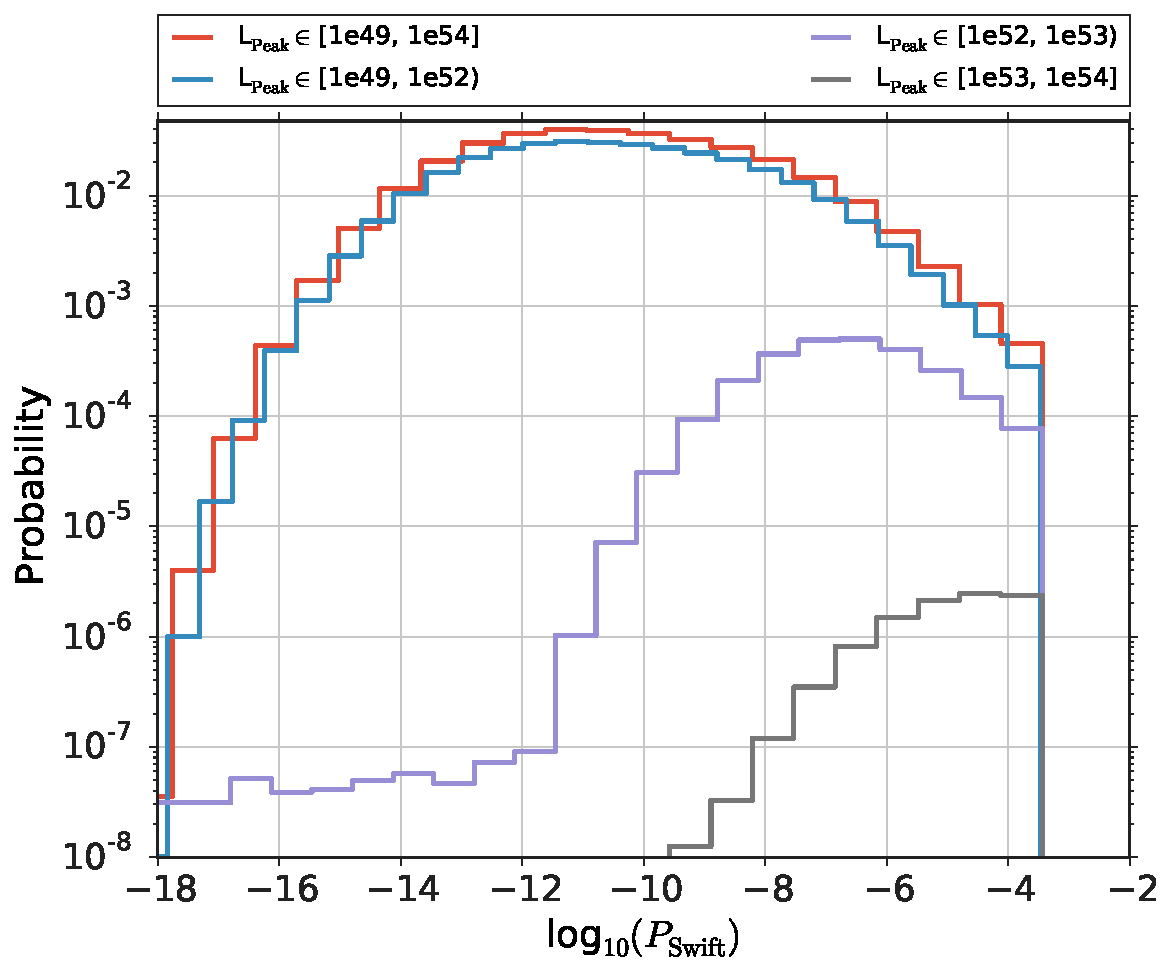
\includegraphics[width=0.45\textwidth]{%
fig/ngrb_hc_lum_dependence_swiftdoublet_ndetF.pdf}}
\caption{The probability for a GRB to have a certain probability to produce a 
Swift doublet. The contribution of the whole signal and the contribution of 
various redshift and luminosity bins are shown. Note that contributions with 
very small 
probabilities ($P_\mathrm{Swift}$) were cut off to display the more relevant 
region.}
\end{figure}

In Figure \ref{fig:ngrb_redshift_dependence_swiftdoublet_ndetF}, one can see 
the probability of a GRB to have a certain probability $P_\mathrm{Swift}$ for a 
swift doublet to be detected. Most GRBs are in a redshift range between 2 and 4 
which corresponds to the peak in the redshift distribution in Figure 
\ref{fig:GRB_rate_density}. However, these GRBs and the GRBs further out mostly 
contribute to the distribution for low to intermediate $P_\mathrm{Swift}$ 
values. The most likely GRBs to be seen in IceCube with high $P_\mathrm{Swift}$ 
values are within a redshift of one even though they occur less frequent due 
to the small volume. In total, about 0.3 GRBs per year are expected to be 
detectable with Swift doublets within the BDT season. About 35\% of which would 
be within the first redshift bin (Figure 
\ref{fig:ngrb_redshift_dependence_swiftdoublet_cum}). However, the other 
regions all contribute more than 10\% to the total signal as well.

\begin{figure}[h]
\centering
 \captionsetup{width=.9\textwidth}
%  \captionsetup{margin=0pt}
\subfloat[WP model\label{fig:ngrb_redshift_dependence_swiftdoublet_cum}]{%
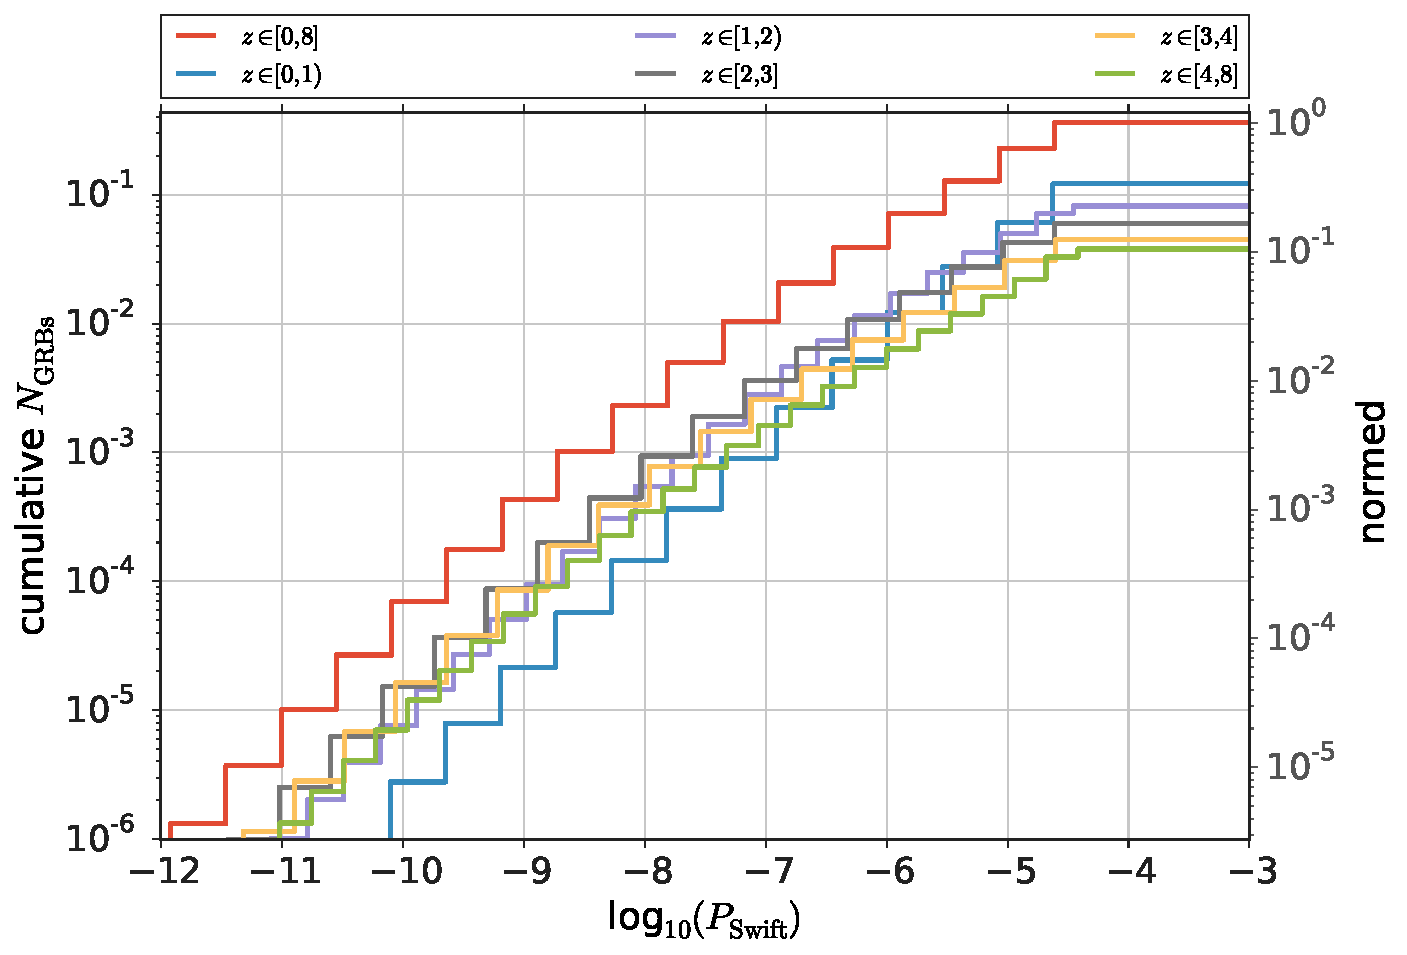
\includegraphics[width=0.45\textwidth]{%
fig/ngrb_redshift_dependence_swiftdoublet_cum.pdf}}
\subfloat[HC model\label{
fig:ngrb_hc_redshift_dependence_swiftdoublet_cum}]{%
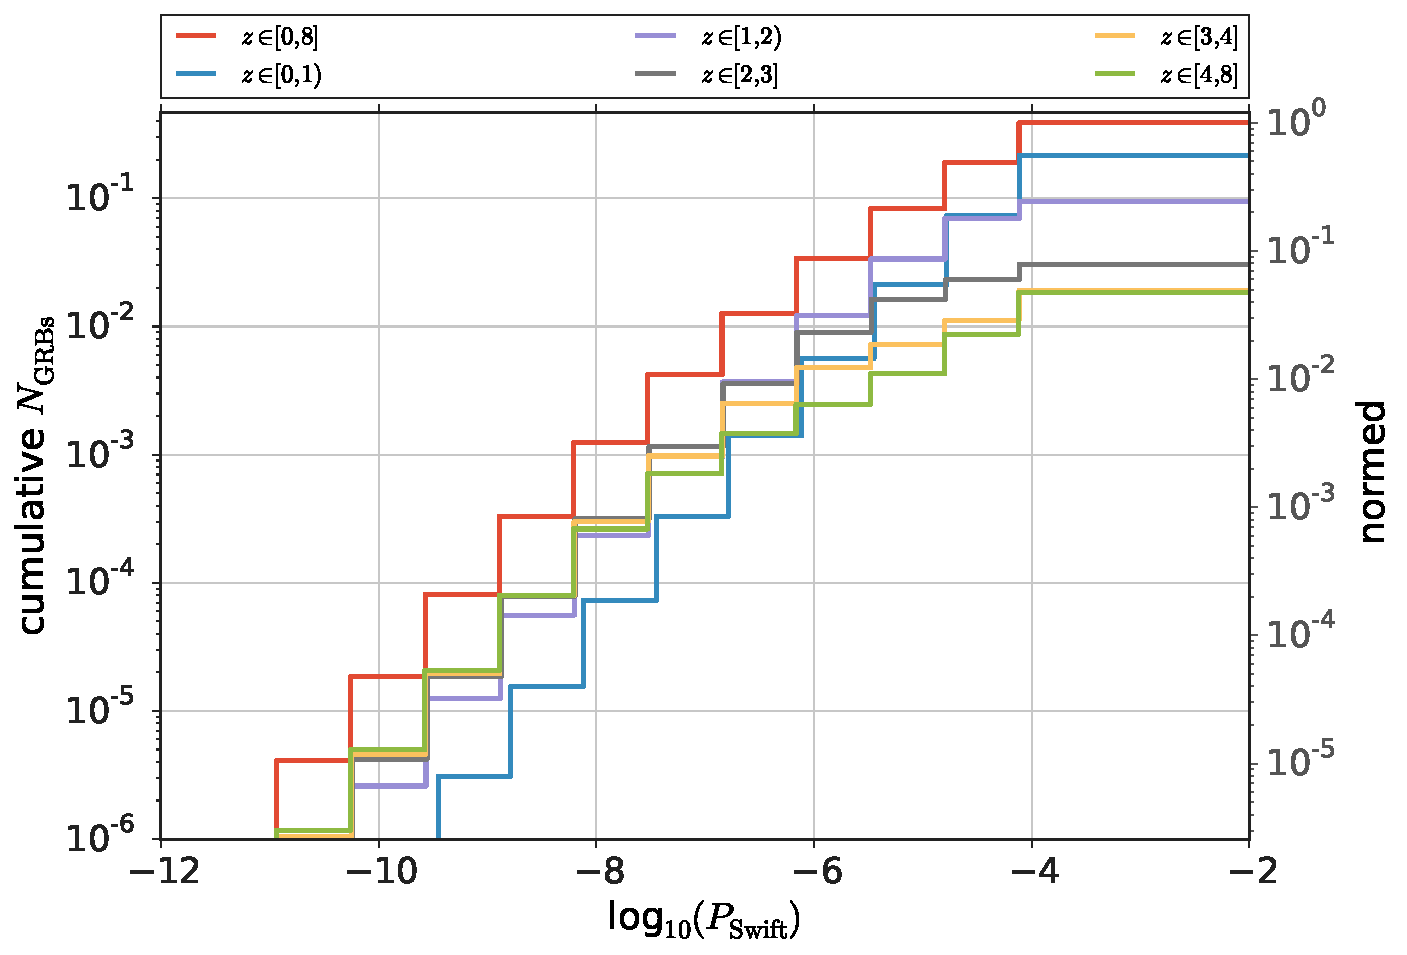
\includegraphics[width=0.45\textwidth]{%
fig/ngrb_hc_redshift_dependence_swiftdoublet_cum.pdf}}\\
\subfloat[WP model\label{fig:ngrb_lum_dependence_swiftdoublet_cum}]{%
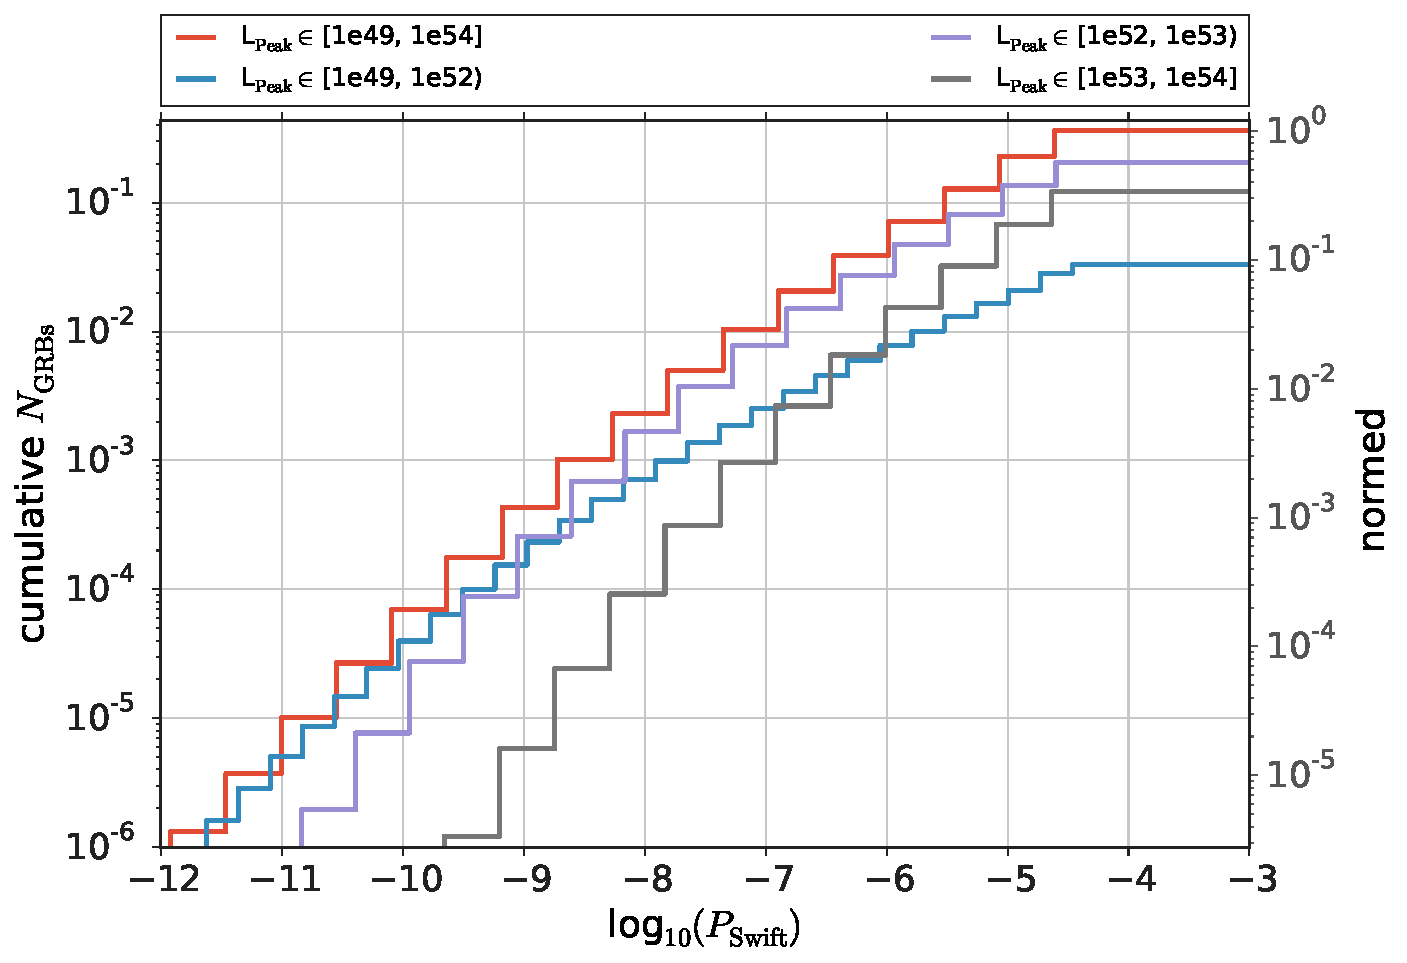
\includegraphics[width=0.45\textwidth]{%
fig/ngrb_lum_dependence_swiftdoublet_cum.pdf}}
\subfloat[HC model\label{fig:ngrb_hc_lum_dependence_swiftdoublet_cum}]{%
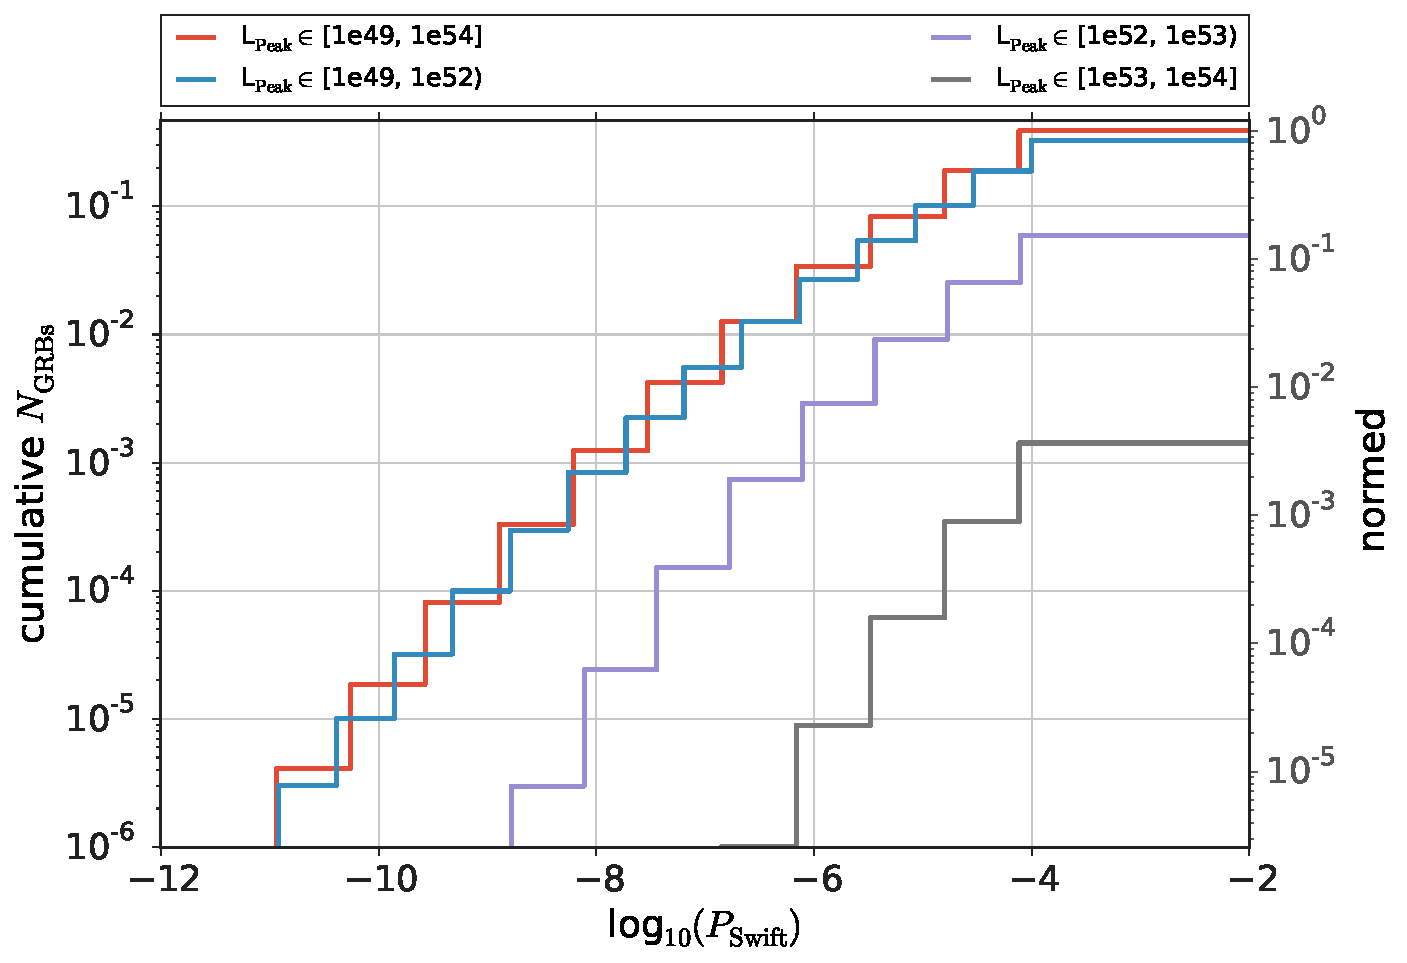
\includegraphics[width=0.45\textwidth]{%
fig/ngrb_hc_lum_dependence_swiftdoublet_cum.pdf}}
\caption{The cumulative distribution to the number of GRBs detected 
per year depending on the probability to produce a Swift doublet. The 
contribution of the whole signal and the contribution of 
various redshift and luminosity bins are shown. On the right 
y-axis, the values are divided by the complete number of GRBs produced per 
year, thus, showing the fraction contributed by the different bins. Note that 
contributions with very small 
probabilities ($P_\mathrm{Swift}$) were cut off to display the more relevant 
region.}
\end{figure}

Similar plots can be examined in Figures 
\ref{fig:ngrb_lum_dependence_swiftdoublet_ndetF} and 
\ref{fig:ngrb_lum_dependence_swiftdoublet_cum} examining the influence of the 
peak luminosity. Low luminosity GRBs of less than $10^{52}\mathrm{ erg / s}$ 
produce mainly GRBs with low detection probability only contributing about 10\% 
to the expected number of detectable GRBs. The main contribution of almost 60\% 
stems from GRBs with peak luminosities within $10^{52}$ and 
$10^{53}\mathrm{erg/s}$ by compromising between abundance and brightness. 
However, this describes the cumulative contribution of all GRBs, the most 
likely GRBs to be actually detectable are very bright and very close GRBs. 
Unfortunately, they happen rather seldom.

The same comparison can be done for the probability to see higher multiplets 
of at least three neutrinos (Figures 
\ref{fig:ngrb_redshift_dependence_multiplet_cum} and 
\ref{fig:ngrb_lum_dependence_multiplet_cum}). The signal is more dependent on 
the very bright and close GRBs as others do not produce the necessary flux to 
make a detection likely. The contribution to the total number of 0.5 detectable 
GRBs per year with the BDT season setup drops to about 6\% for the low 
luminosity GRBs while the very close GRBs up to a redshift of one constitute 
about 80\% of the total signal for higher multiplets.


\begin{figure}[h]
\centering
 \captionsetup{width=.9\textwidth}
%  \captionsetup{margin=0pt}
\subfloat[WP model\label{fig:ngrb_lum_dependence_multiplet_cum}]{%
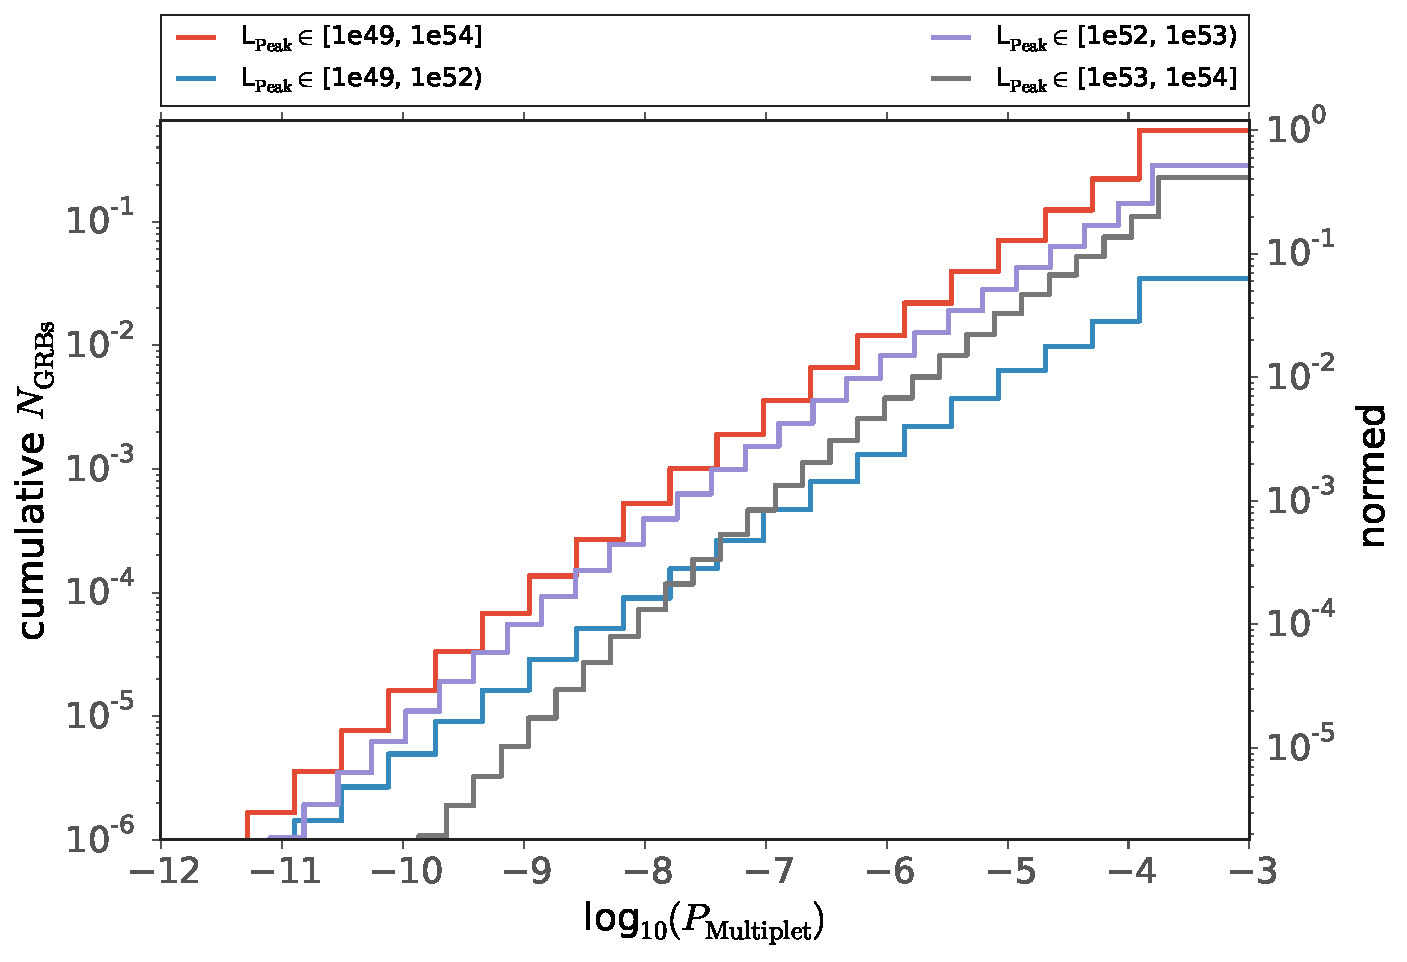
\includegraphics[width=0.45\textwidth]{%
fig/ngrb_lum_dependence_multiplet_cum.pdf}}
\subfloat[HC model\label{fig:ngrb_hc_lum_dependence_multiplet_cum}]{%
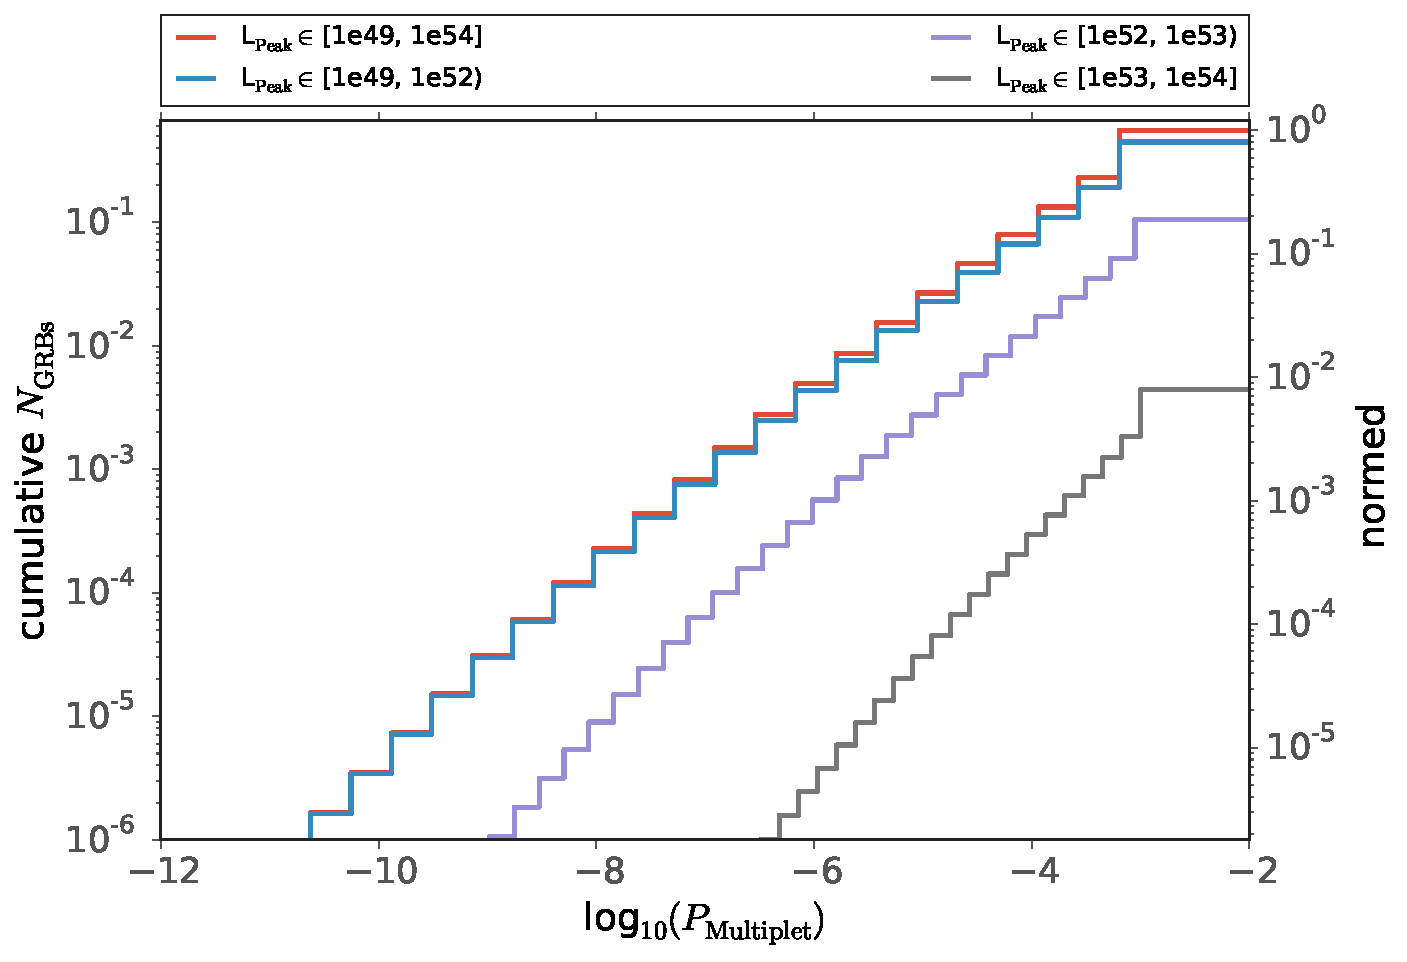
\includegraphics[width=0.45\textwidth]{%
fig/ngrb_hc_lum_dependence_multiplet_cum.pdf}}\\
\subfloat[WP model\label{fig:ngrb_redshift_dependence_multiplet_cum}]{%
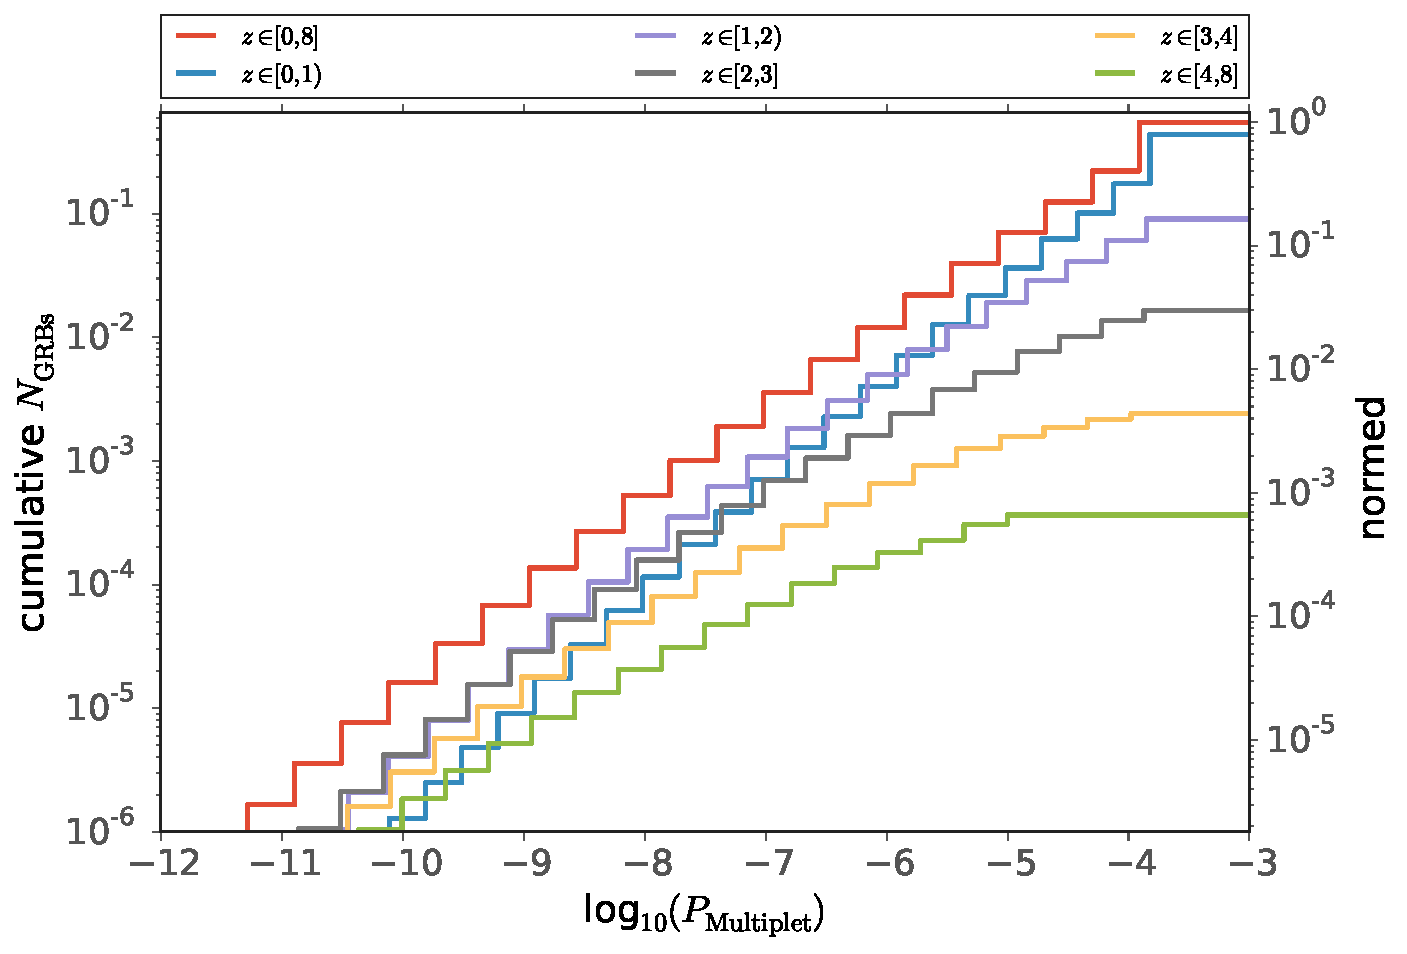
\includegraphics[width=0.45\textwidth]{%
fig/ngrb_redshift_dependence_multiplet_cum.pdf}}
\subfloat[HC model\label{fig:ngrb_hc_redshift_dependence_multiplet_cum}]{%
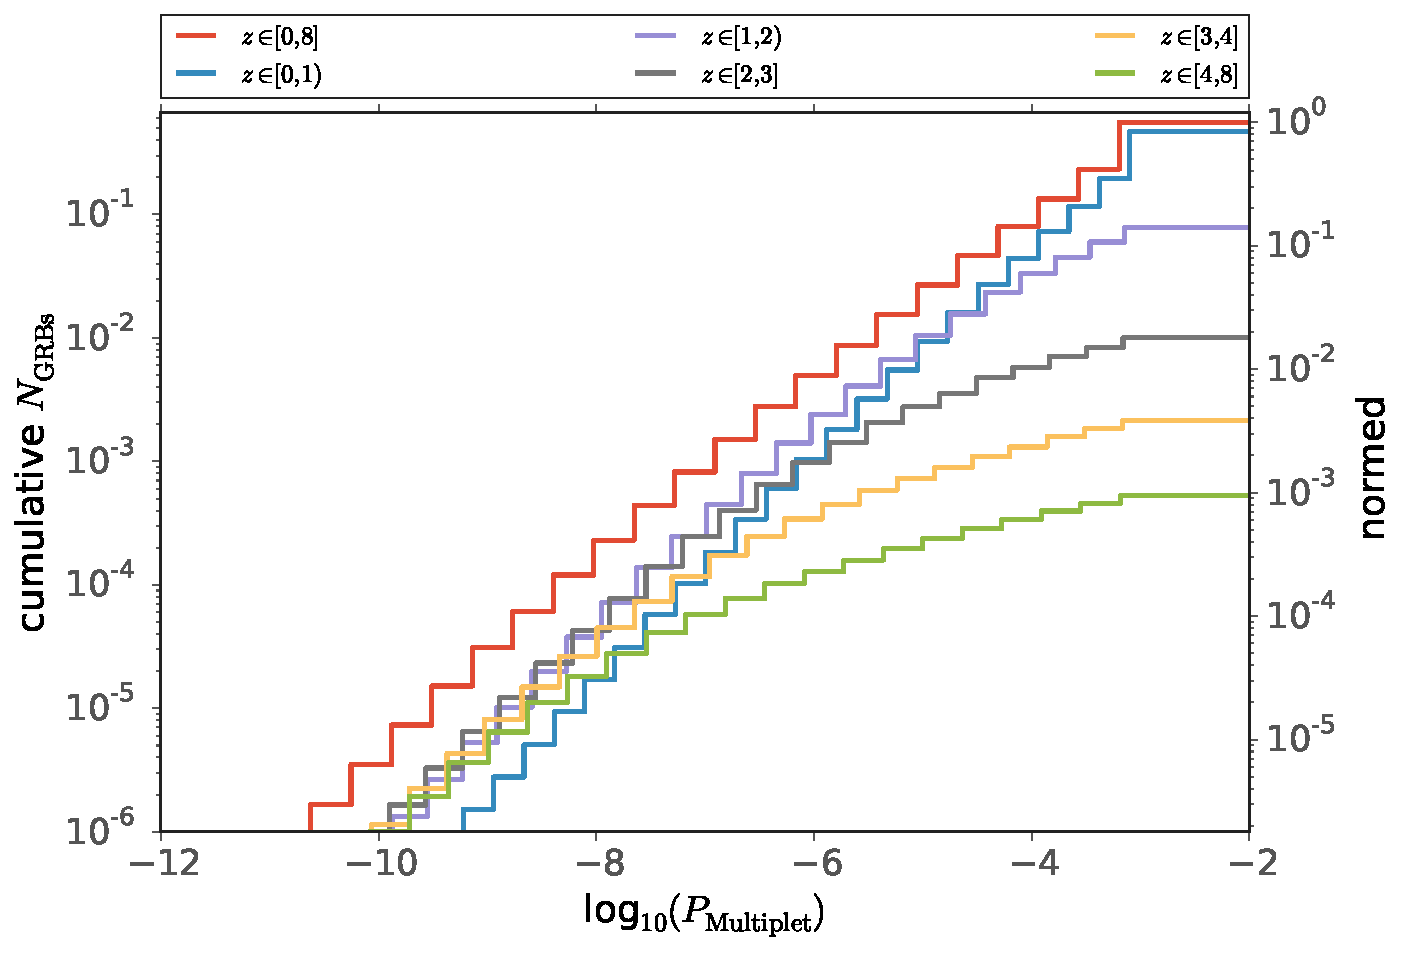
\includegraphics[width=0.45\textwidth]{%
fig/ngrb_hc_redshift_dependence_multiplet_cum.pdf}}
\caption{The cumulative distribution to the number of GRBs detected 
per year depending on the probability to produce a higher multiplet. The 
contribution of the whole signal and the contribution of 
various luminosity and redshift bins are shown. On the right 
y-axis, the values are divided by the complete number of GRBs produced per 
year, thus, showing the fraction contributed by the different bins. Note that 
contributions with very small 
probabilities ($P_\mathrm{Multiplet}$) were cut off to display the more 
relevant region.}
\end{figure}


Combining these results, one can see that we expect most signal from the 
very rare and close GRBs within a redshift of one. The number of detectable 
GRBs per year is displayed over the redshift in Figure
\ref{fig:hfcws_g2p3_n0p0595}. Both channels - the detection with swift doublets 
and higher multiplets - peak in the number of GRBs per year for GRBs within the 
first redshift bin with the multiplets dominating the signal strength. GRBs at 
these ranges produce a neutrino flux high enough that it is more likely to see 
multiplets than swift doublets. Exploring the cosmos to higher redshifts, the 
flux decreases and starting at about $z=1$ it is more likely to see swift 
doublets. However, the chance to be seen at all decreases as well, limiting the 
contribution to the cumulative signal with anything above $z=2$ only summing up 
to about 1\% of the combined multiplet and swift doublet signal. Combined with 
the fact that in contrast to the doublets there is very limited multiplet 
background, the higher multiplet channel is the main contributer to the 90\% 
confidence point for an expected 3000 GRBs per year. 

\begin{figure}[h]
\centering
 \captionsetup{width=.9\textwidth}
%  \captionsetup{margin=0pt}
\subfloat[WP model\label{fig:hfcws_g2p3_n0p0595}]{%
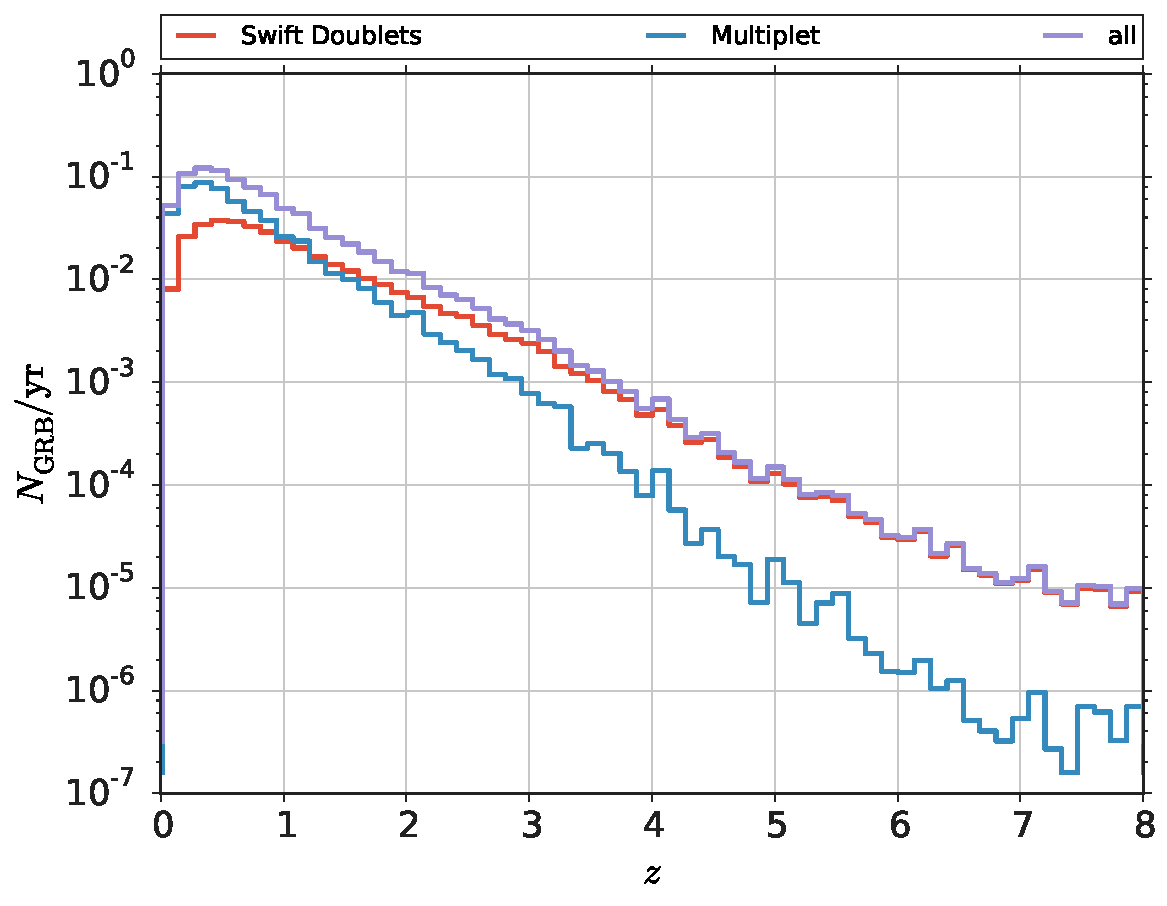
\includegraphics[width=0.45\textwidth]{%
fig/hfcws_g2p3_n0p0595.pdf}}
\subfloat[HC model\label{fig:hfcws_g2p3_hc2_n0p0759}]{%
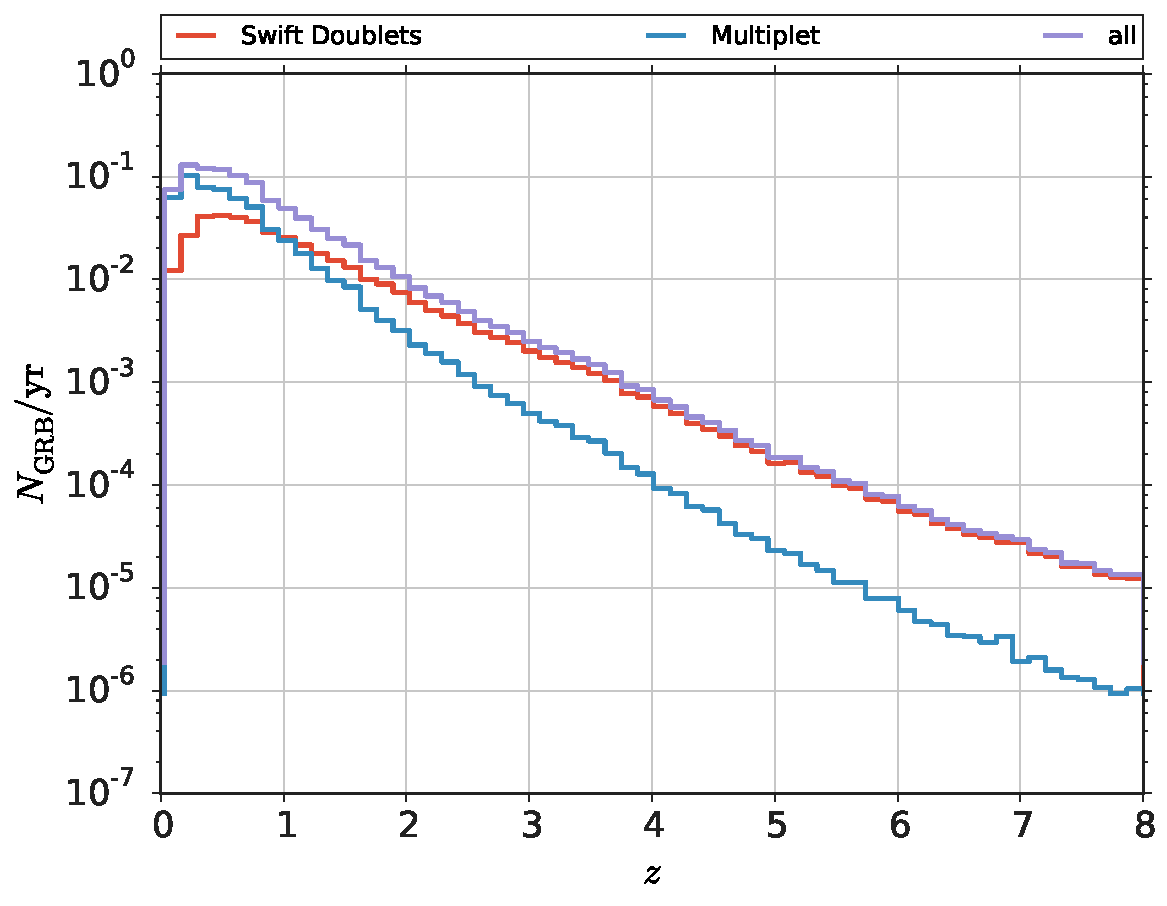
\includegraphics[width=0.45\textwidth]{%
fig/hfcws_g2p3_hc2_n0p0759.pdf}}
\caption{The cumulative distribution to the number of GRBs detected 
per year depending on the probability to produce a higher multiplet. The 
contribution of the whole signal and the contribution of 
various luminosity and redshift bins are shown. On the right 
y-axis, the values are divided by the complete number of GRBs produced per 
year, thus, showing the fraction contributed by the different bins. Note that 
contributions with very small 
probabilities ($P_\mathrm{Multiplet}$) were cut off to display the more 
relevant region.}
\end{figure}

Reducing the fraction of contribution to the HESE flux by GRBs, reduces the 
flux per GRB and as such the importance of the multiplet channel as well. A 
similar effect is to be expected by looking at higher rate densities. With more 
sources producing the same diffuse neutrino flux, the flux per source decreases.


% test statistic distribution shows the point at which p=0.9 was reached for WP 
% for 3000 GRBs showing maximum contribution of 0.05\%??? (factor 0.05 on HESE 
% flux -> $\mu$ <- describing the scaling in )
% 
% total number of GRBs is uncertain. therefore limits depending on the transient 
% rate density and the fraction of the HESE flux are drawn. the more sources 
% contribute to the known signal the less flux can be attributed to one source. 
% scale $\mu (Nexp) = \mu \frac{x GRBs}{3000 GRBs}$ . limit plots
% 
% the softer the spectrum the more singlets (especially at low energies) and 
% therefore more multiplets (reference spectrum plot) can be expected. 
% influence of a minimal energy cutoff in section ???. best limit for gamma=2.7 
% scenario. worst for gamma=2. with cutoff. some numbers (maybe in table)
% 
% looking at higher transient rates, limits extend to SN (which kind) especially 
% considering that not all SN are expected to generate jets. further discussion 
% in section ???.
% 
% where does signal come from? close and high. need to see plots to write more



\subsection{Different models}
So far, the Wanderman Piran model was examined to present the results of the
analysis. The influence of two different factors will be analyzed in the 
subsequent sections. 

The WP model is based on a broad luminosity function. The resulting variation 
in luminosity can lead to seldom but very bright GRBs producing the most 
detectable signal. Two different luminosity functions will be examined, the 
Howell Coward model (Section \ref{sec:results_HC}) and a more SN conform 
luminosity distribution (Section \ref{sec:results_SN}). 

The second factor is a low energy cut-off, having great influence on the final 
limits on the HESE flux contribution (Section \ref{sec:results_Emin}).

\subsubsection{Howell Coward}
\label{sec:results_HC}
% discripancy higher at high rates between models? at low not so much because 
% mainly dependent on multiplets and therefore close GRBs?
The Howell Coward model (Section ???) predicts various luminosity distributions 
that have one thing in common when compared to WP: less GRBs are predicted at 
high peak luminosity values (Fig. \ref{fig:wp_hc_comp_lum}). While the slope 
at 
low peak luminosities is with $\alpha_{WP}=-0.17$ and $\alpha_{HC}=-0.13$ quite 
similar, the distributions diverge quite strongly above $L_\mathrm{Peak} \geq 
1e52 \mathrm{ erg} \mathrm{ s}^{-1}$ and the HC luminosity function drops with 
$\beta{HC}=-2.42$ much faster than the WP function ($\beta{WP}=-1.44$).
% \begin{figure}[h]
% \centering
%  \captionsetup{width=.9\textwidth}
% %  \captionsetup{margin=0pt}
% \subfloat[WP model\label{fig:test_statistic_norm0p0595_rate3e3}]{%
% 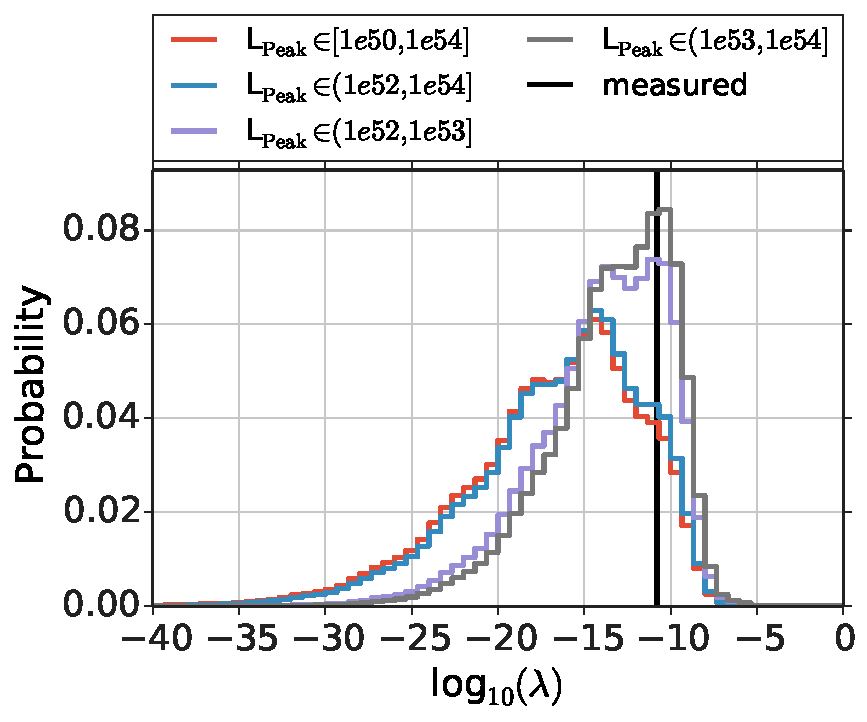
\includegraphics[width=0.45\textwidth]{%
% fig/test_statistic_norm0p0595_rate3e3.pdf}}
% \subfloat[HC model\label{fig:test_statistic_hc_norm0p0759_rate3e3}]{%
% 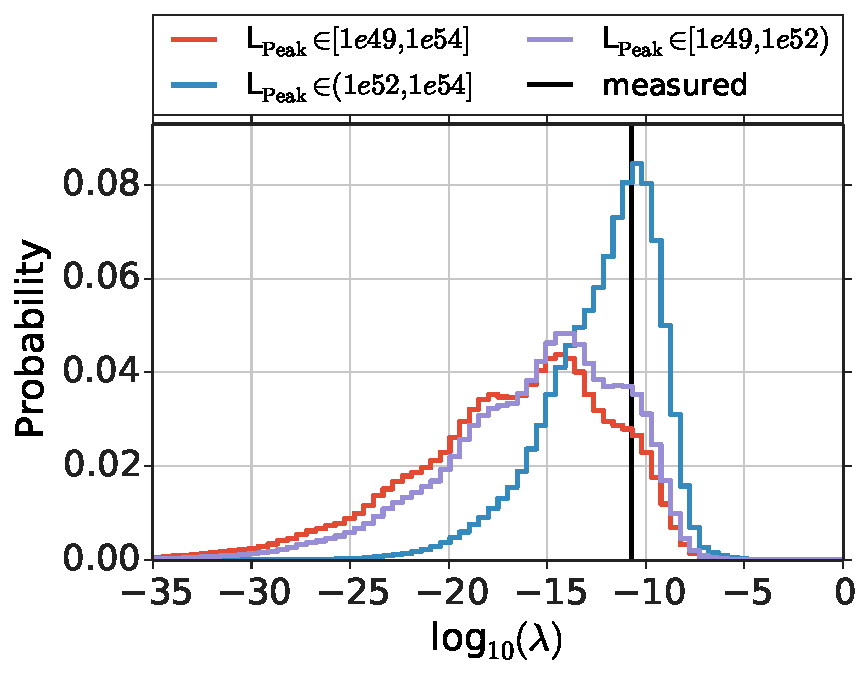
\includegraphics[width=0.45\textwidth]{%
% fig/test_statistic_hc_norm0p0759_rate3e3.pdf}}
% \caption{caption}
% \end{figure}



The impact of this deviating behavior will be examined for the flux model with 
a spectral index of $\gamma=2.3$ as the intermediate model. The result can be 
seen in Figure \ref{fig:limits_wphc_g2p3} displaying the less 
stringent limits of the HC model. 
Assuming 3000 contributing GRBs per year, the contribution to the HESE flux of 
GRBs following the HC luminosity can be determined at a 90\% confidence level to 
be less than 7.59\% (WP: 5.95\%). This point will be examined in more detail in 
the following paragraphs.

\begin{figure}[h]
\centering
 \captionsetup{width=.9\textwidth}
%  \captionsetup{margin=0pt}
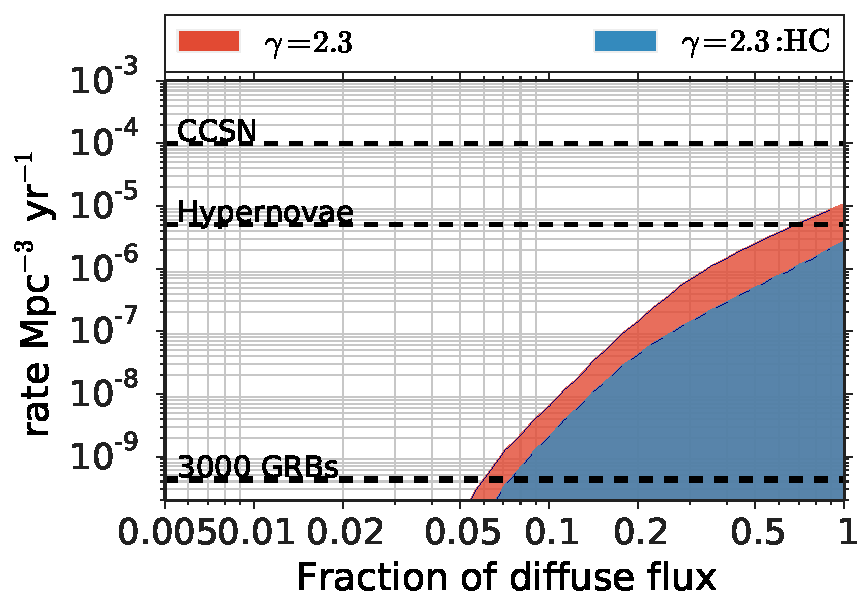
\includegraphics[width=0.75\textwidth]{%
fig/limits_wphc_g2p3.pdf}
\caption{Limits on the contribution of short transient sources to the HESE 
flux depending on their rate density. The 90\% confidence regions are shown for 
a spectrum with $\gamma=2.3$ comparing the WP and the HC model.}
\label{fig:limits_wphc_g2p3}
\end{figure}

Looking at the luminosity distribution (Fig. \ref{fig:wp_hc_comp_lum}) already 
indicates that high luminosity GRBs will have less impact for the HC model than 
the WP model as they are suppressed in frequency by almost four orders of 
magnitude at the highest luminosities of $10^{54}\mathrm{erg/s}$ alone. Figure 
\ref{fig:ngrb_hc_lum_dependence_swiftdoublet_ndetF} demonstrates that the low 
luminosity GRBs dominate the whole range of detection probabilities 
($P_\mathrm{Swift}$) even to the highest values contributing a total of about 
90\% to the cumulative swift doublet signal (Fig. 
\ref{fig:ngrb_hc_lum_dependence_swiftdoublet_cum}). The other GRBs mainly occur 
at high probability values but lack influence nonetheless due to their 
sparsity. 

Not having the abundance of bright GRBs to produce high neutrino fluxes even at 
great distances, the cumulative swift doublet signal depends with almost 60\%  
on GRBs within a redshift of one (WP: 35\%).  % \begin{figure}[h]

In case of the higher multiplets, the signal contribution is similar dependent 
on the low luminosity GRBs (Fig. 
\ref{fig:ngrb_hc_lum_dependence_multiplet_cum}) and even more so on the close 
ones (Fig. \ref{fig:ngrb_hc_redshift_dependence_multiplet_cum}). However, while 
 the behavior so far differed quite obviously from the distribution produced 
with the WP model, the possibility to detect a 
neutrino multiplet depends similarly on close by GRBs (compare Figs. 
\ref{fig:ngrb_hc_redshift_dependence_multiplet_cum} and 
\ref{fig:ngrb_redshift_dependence_multiplet_cum}). Keeping in mind that most of 
the signal is generated by multiplets within a redshift of one for both the WP 
model (Fig \ref{fig:hfcws_g2p3_n0p0595}) and the HC model (Fig. 
\ref{fig:hfcws_g2p3_hc2_n0p0759}), the comparatively small difference of a 
factor of 1.28 between the two points of 90\% confidence level assuming 3000 
GRBs per year is explained. The lack of high luminosity GRBs in the HC model 
does not matter, as the signal depends mainly on GRBs close enough to produce 
enough higher multiplets.
The discrepancy between the two models increase slightly towards higher GRB 
rate densities with less flux per GRB. While the flux decrease can be 
compensated to a degree by the high luminosity GRBs, this is not possible for 
the HC model.

% \centering
%  \captionsetup{width=.9\textwidth}
% %  \captionsetup{margin=0pt}
% \subfloat[WP model\label{
% fig:test_statistic_norm0p0595_rate3e3_cum}]{%
% 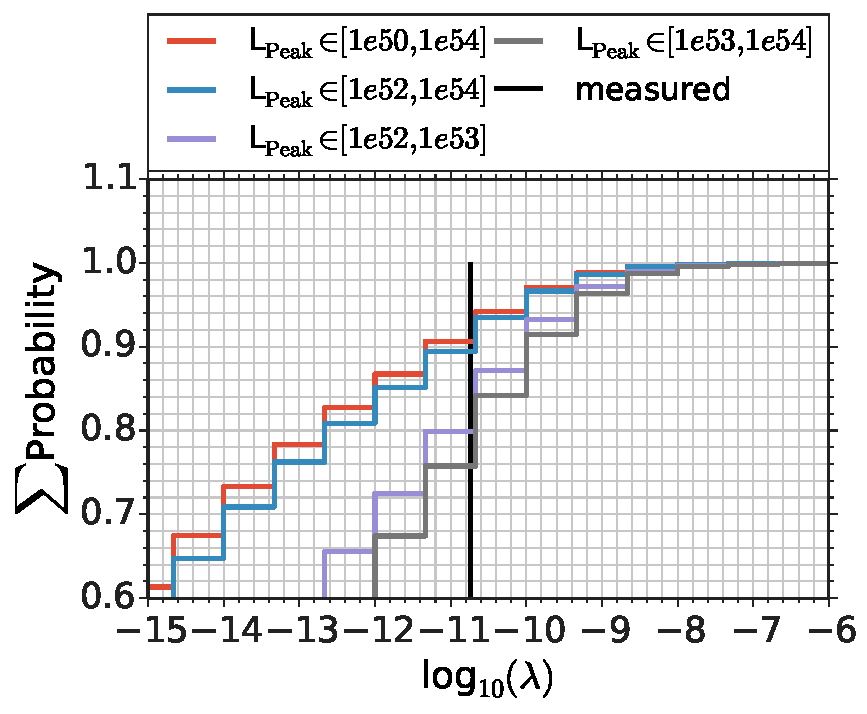
\includegraphics[width=0.45\textwidth]{%
% fig/test_statistic_norm0p0595_rate3e3_cum.pdf}}
% \subfloat[HC model\label{
% fig:test_statistic_hc_norm0p0759_rate3e3_cum}]{%
% 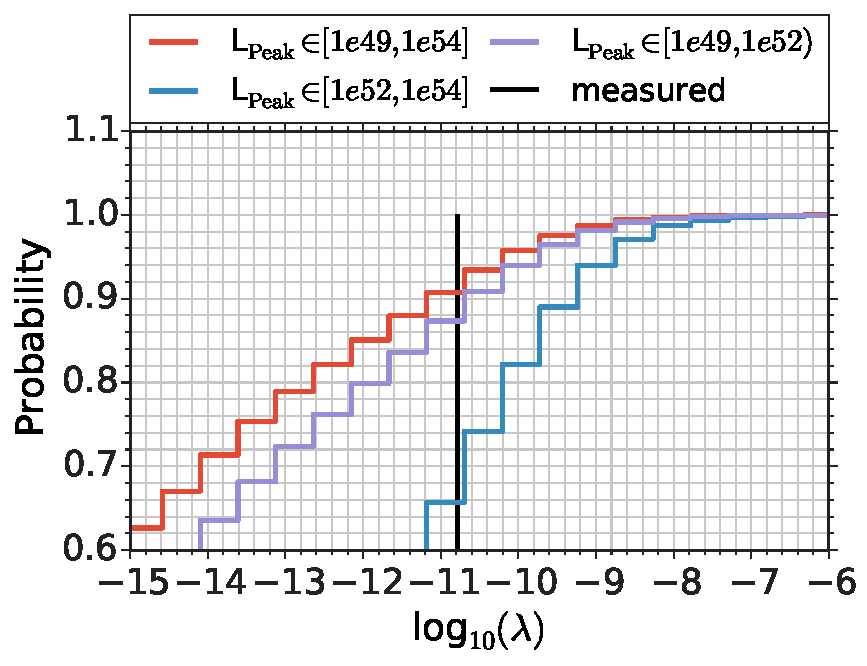
\includegraphics[width=0.45\textwidth]{%
% fig/test_statistic_hc_norm0p0759_rate3e3_cum.pdf}}
% \caption{caption}
% \end{figure}

% Looking at the test statistic distributions at the 90\% exclusion value for 
% each model, the low luminosity GRBs reproduce the overall distribution quite 
% well (Fig. ???) in case of the HC model while one can observe a significant 
% shift between the distributions - and therefore worse limits - for the WP model 
% (Fig. ???). The cumulative distributions further support the result that the 
% high luminosity GRBs do not contribute much to the HC-limit while each 
% luminosity bin ($L_\mathrm{Peak} \in [1e52, 1e53)$ and $L_\mathrm{Peak} \in 
% [1e53, 1e54]$) can still rule out the WP model at about
% 80\% confidence level.


% show contribution to Luminosity, redshift??? maybe how far can I look -> more 
% dependent on low lum GRBs. can not look as deep.

In conclusion it is possible to say that the limits for do only depend 
partially on the luminosity 
function. The limits on the HC model are mainly produced by the low 
luminosity GRBs due to the lack of high luminosity ones. This leads to 
worse limits in comparison to the WP model. However, the discrepancy is 
contained due to the dependence on multiplets from close by GRBs. Both 
models still exclude a wide 
region of parameter space.


\subsubsection{Supernova Luminosity Function}
\label{sec:results_SN}
% redshift distribution can stay the same. or did I already write that?
Examining a different luminosity distribution in the previous section was 
interesting, as a big variation of the luminosity could lead to the one very 
bright GRB to be detected. Limiting the number of high luminosity GRBs 
worsened the limits but a wide range of the parameter space could still be 
ruled out. Continuing the process one could slim down the luminosity 
distribution until only a delta function remains. The SN luminosity function 
(Eq. ???) is a step in that direction with a Gaussian with width ???. The 
average luminosity is higher than a lot of values from the WP or HC models, 
however, it is very unlikely to have GRBs with very high luminosities.

SNe are especially interesting because using the WP model and a spectrum with 
$\gamma=2.7$, the limits extend from rate densities that are likely for GRBs to 
very high values and reaching the population of Core Collapse SNe. According to 
???, some SNe could create jets similar to GRBs producing high energy 
neutrinos. Considering that not all SNe might have a jet and that we could only 
see them if the jet pointed towards earth, one has to look at the parameter 
space at possibly a hundredth or less than the actual SN rate density making 
the limits even more stringent. Using the same redshift distribution as 
motivated in Section ??? and the luminosity distribution (Eq. ???) chosen to 
represent the SNe population, the limits worsen but still exclude the 
possibility that SNe contribute the complete measured high energy neutrino 
flux (Fig. \ref{fig:limits_wpsn_g2p7}). However, this depends on choosing the 
most optimistic fit to the measured HESE flux with $\gamma=2.7$ (Eq. ???). 
Using a harder spectrum decreases the chance of ruling out SNe as the main 
source.

\begin{figure}[h]
\centering
 \captionsetup{width=.9\textwidth}
%  \captionsetup{margin=0pt}
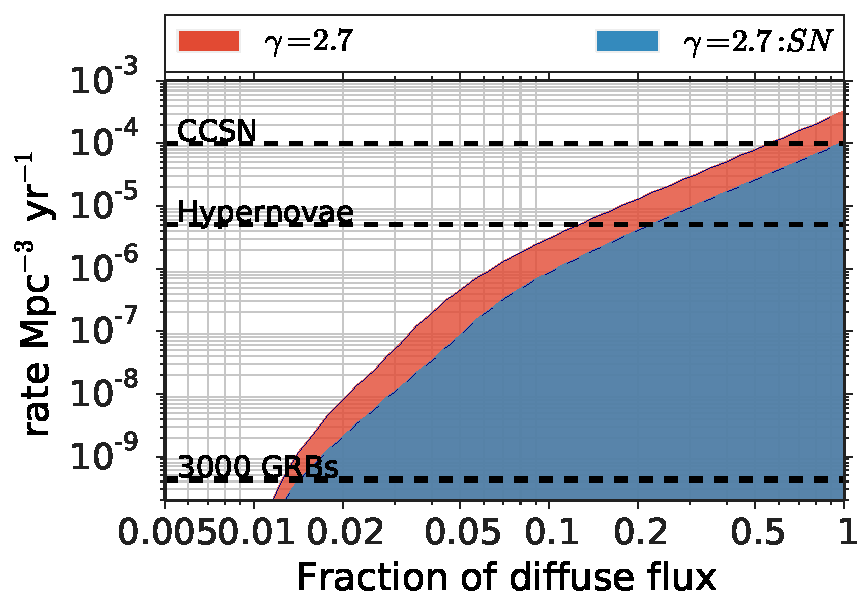
\includegraphics[width=0.75\textwidth]{%
fig/limits_wpsn_g2p7.pdf}
\caption{Limits on the contribution of short transient sources to the HESE 
flux depending on their rate density. The 90\% confidence regions are shown for 
a spectrum with $\gamma=2.7$ comparing the WP model to a more SN like 
luminosity distribution.}
\label{fig:limits_wpsn_g2p7}
\end{figure}

\subsubsection{Low Energy Cut-Off}
\label{sec:results_Emin}
This section examines the influence low energy cut-off, the minimal energy 
neutrinos have at source (Eq. ???) that arises in the flux calculation (Eq. 
???). As explained in section ???, the absolute normalization of the flux does 
not change but stays the same when using the same spectrum. However, if the 
cut-off is high enough, no low energy neutrino is available to form multiplets 
reducing the likelihood of detection. 

The lowest measured energy of the HESE events was 30 TeV. Setting 
$\hat{E}_\mathrm{min}$ to 100 TeV, no OFU singlet with energies lower than ??? 
GeV should contribute (??? line in Fig. ???). The impact on the signal is more 
pronounced for the softer spectra, as they predict more events at lower 
energies (Fig. ???). Using the spectrum with $\gamma=2.3$, the limits worsen 
drastically and are in the range of the spectrum with $\gamma=2$ with an 
exponential cut-off (Fig. \ref{fig:limits_wp_g2p3_g2p0_Emin100e3}). 

% word about should be same for E-2 as OFU spectra are not that different above 
% that energy


\begin{figure}[h]
\centering
 \captionsetup{width=.9\textwidth}
%  \captionsetup{margin=0pt}
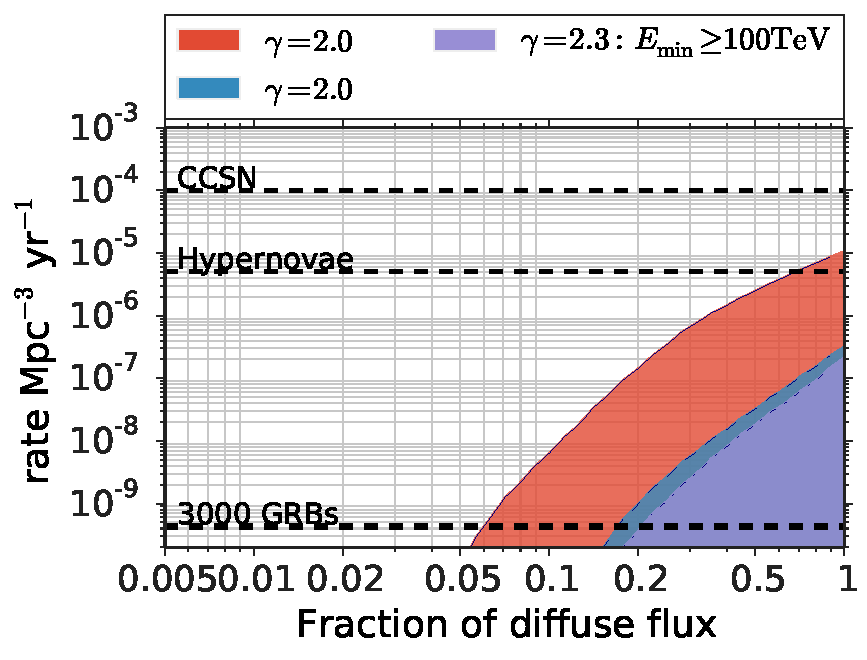
\includegraphics[width=0.75\textwidth]{%
fig/limits_wp_g2p3_g2p0_Emin100e3.pdf}
\caption{Limits on the contribution of short transient sources to the HESE 
flux depending on their rate density. The 90\% confidence regions are shown for 
a spectrum with $\gamma=2.3$ and $\gamma=2$ comparing them to a spectrum with 
$\gamma=2.3$ and a minimal neutrino energy at source of 100 TeV.}
\label{fig:limits_wp_g2p3_g2p0_Emin100e3}
\end{figure}


